\documentclass[11pt]{article}

\usepackage[utf8]{inputenc}
\usepackage{amsmath}
\usepackage{graphicx}
\usepackage{enumerate}
\usepackage{subcaption}
\usepackage{hyperref}
\usepackage{hypcap}
\usepackage{relsize}
\usepackage{caption}
\usepackage{array} 
\usepackage[margin=1in, paperwidth=8.5in, paperheight=11in]{geometry}
\usepackage{float}
\usepackage{array}
\usepackage{tabularx}
\usepackage{textgreek}
\usepackage{amsmath}
\usepackage{amssymb}
\usepackage{amsthm}
\usepackage{parskip}
\usepackage{svg}
\usepackage{blindtext}
\usepackage{listings}
% \hypersetup{
%     colorlinks=true,
%     linkcolor=blue,
%     filecolor=magenta,
%     urlcolor=cyan,
% }
\lstset{
  basicstyle=\ttfamily,
  columns=fullflexible,
  % frame=single,
  breaklines=true,
  postbreak=\mbox{\textcolor{red}{$\hookrightarrow$}\space},
}

\usepackage{graphicx}
\title{Miniproject 1: CMOS AND Gate}
\author{Drew Pang }
\date{22 September, 2025}

\begin{document}

\maketitle

\section*{Schematic Capture and Simulation}

\subsection*{Inverter}

\begin{figure}[H]
  \centering
  \includesvg[inkscapelatex=false,width=5cm]{media/inverter_sch.svg}
  \includesvg[inkscapelatex=false,width=5cm]{media/inverter_sym.svg}
  \caption{CMOS inverter schematic and symbol}
\end{figure}

My CMOS inverter was constructed as a classical CMOS inverter using one NMOS and one PMOS transistor. The width and length were set in anticipation of creating minimum size transistors.

\subsection*{NAND Gate}

\begin{figure}[H]
  \centering
  \includesvg[inkscapelatex=false,width=8cm]{media/nand_sch.svg}
  \includesvg[inkscapelatex=false,width=5cm]{media/nand_sym.svg}
  \caption{CMOS NAND gate schematic and symbol}
\end{figure}

I created a CMOS NAND gate using two NMOS and two PMOS transistors. Importantly, the bulk of both NMOS transistors are tied to ground to properly bias the body-source and body-drain diodes.

\subsection*{AND Gate}

\begin{figure}[H]
  \centering
  \includesvg[inkscapelatex=false,width=8cm]{media/and_sch.svg}
  \includesvg[inkscapelatex=false,width=5cm]{media/and_sym.svg}
  \caption{CMOS AND gate schematic and symbol}
\end{figure}

Using the inverter and NAND gate, an AND gate can be constructed by inverting the output of the NAND gate.

\subsection*{AND Transient Simulation}

\begin{figure}[H]
  \centering
  \includesvg[inkscapelatex=false,width=17cm]{media/and_tran.svg}
  \caption{CMOS AND gate schematic and symbol}
\end{figure}

My AND gate was simulated using two square waves with different frequencies. With a 25MHz clock input on A and 12.5MHz clock input on B, the output Y cycles through all possible input combinations. As one would expect, the output is only high when both A and B are high.

\begin{figure}[H]
  \centering
  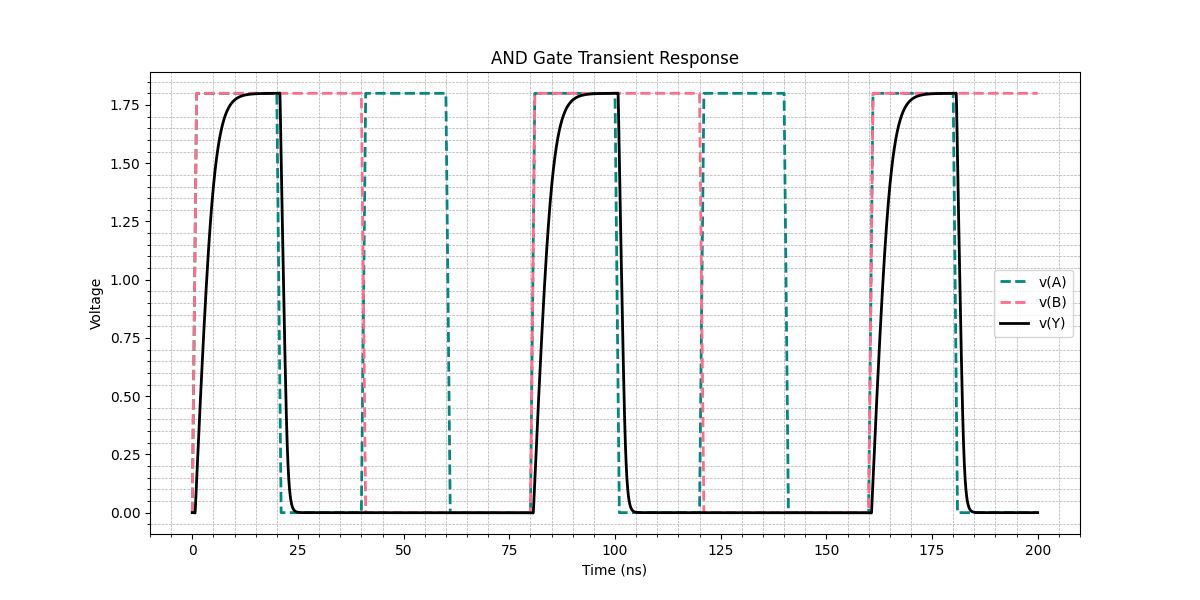
\includegraphics[width=\linewidth]{media/and_tran.png}
  \caption{CMOS AND gate transient response}
\end{figure}

\section*{Layout Design}

\subsection*{Inverter}
\begin{figure}[H]
  \centering
  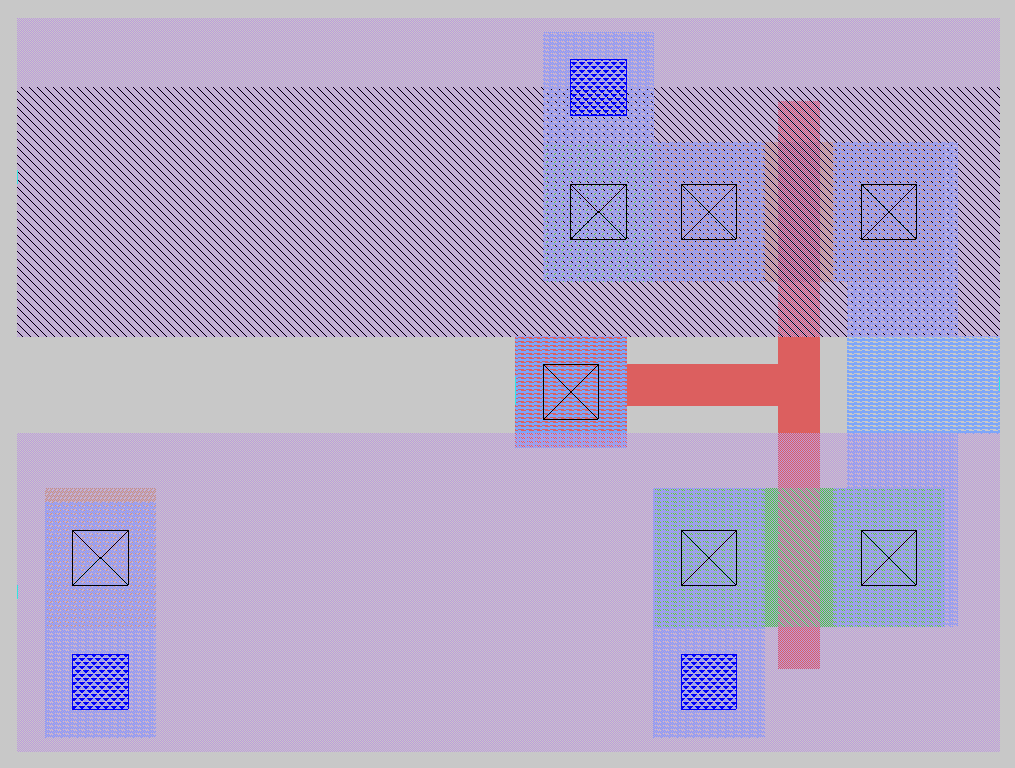
\includegraphics[width=\linewidth]{media/inverter_layout.png}
  \caption{CMOS inverter layout}
\end{figure}

The above inverter does not necessarily follow the standard cell format, but instead was made to fit and overlap with a NAND gate to form a compact AND gate. The inverter input is the center polysilicon contact, and the output is the local interconnect on the right.

\subsection*{NAND}
\begin{figure}[H]
  \centering
  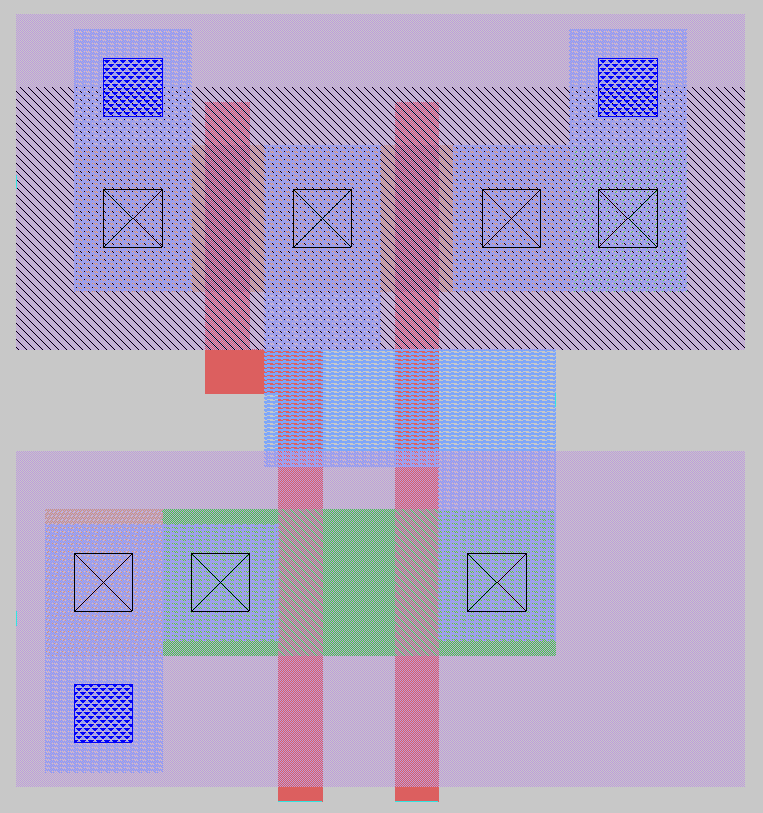
\includegraphics[width=14cm]{media/nand_layout.png}
  \caption{NAND gate layout}
\end{figure}

The above NAND gate follows the move typical standard cell format. The A and B inputs are the polysilcon strips accessible at the bottom, and the output is the local interconnect in the middle.

\subsection*{AND}

\begin{figure}[H]
  \centering
  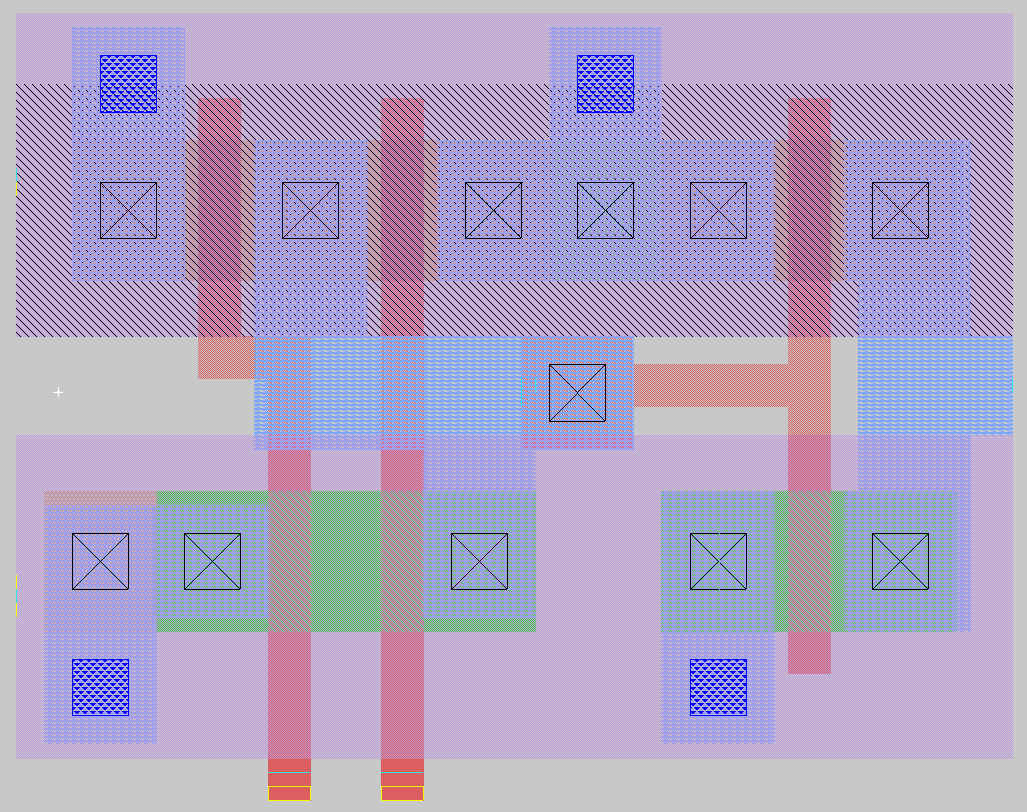
\includegraphics[width=\linewidth]{media/and_layout.png}
  \caption{AND gate layout}
\end{figure}

An AND gate was constructed using the inverter and NAND layouts. Some sections overlap, such as the polysilicon contact in the middle and the P type substrate diffusion. Metal 1 contacts were placed offset from local interconnect contacts, but will be stacked on top of each other in the future. Like the NAND gate, the A and B inputs are accessible at the bottom, and the output is the local interconnect on the right side.

\section*{Layout Versus Schematic}

Netcomp reported matches between my schematic and layout. The Netcomp output and log file can be found in appendix A and B respectively. 




\newpage

\section*{Appendix A: Netcomp Output}
\begin{lstlisting}
Netgen 1.5.300 compiled on Sat Sep 20 09:39:56 PM EDT 2025
Warning: netgen command 'format' use fully-qualified name '::netgen::format'
Warning: netgen command 'global' use fully-qualified name '::netgen::global'
Reading netlist file and.spice
Call to undefined subcircuit sky130_fd_pr__nfet_01v8
Creating placeholder cell definition.
Call to undefined subcircuit sky130_fd_pr__pfet_01v8
Creating placeholder cell definition.
Reading netlist file and_xschem.spice
Call to undefined subcircuit nand
Creating placeholder cell definition.
Call to undefined subcircuit inverter
Creating placeholder cell definition.
Call to undefined subcircuit sky130_fd_pr__nfet_01v8
Creating placeholder cell definition.
Call to undefined subcircuit sky130_fd_pr__pfet_01v8
Creating placeholder cell definition.

Reading setup file /usr/local/share/pdk/sky130A/libs.tech/netgen/sky130A_setup.tcl

Model sky130_fd_pr__nfet_01v8 pin 1 == 3
No property mult found for device sky130_fd_pr__nfet_01v8
No property sa found for device sky130_fd_pr__nfet_01v8
No property sb found for device sky130_fd_pr__nfet_01v8
No property sd found for device sky130_fd_pr__nfet_01v8
No property nf found for device sky130_fd_pr__nfet_01v8
No property nrd found for device sky130_fd_pr__nfet_01v8
No property nrs found for device sky130_fd_pr__nfet_01v8
No property area found for device sky130_fd_pr__nfet_01v8
No property perim found for device sky130_fd_pr__nfet_01v8
No property topography found for device sky130_fd_pr__nfet_01v8
Model sky130_fd_pr__nfet_01v8 pin 1 == 3
No property area found for device sky130_fd_pr__nfet_01v8
No property perim found for device sky130_fd_pr__nfet_01v8
No property topography found for device sky130_fd_pr__nfet_01v8
Model sky130_fd_pr__pfet_01v8 pin 1 == 3
No property mult found for device sky130_fd_pr__pfet_01v8
No property sa found for device sky130_fd_pr__pfet_01v8
No property sb found for device sky130_fd_pr__pfet_01v8
No property sd found for device sky130_fd_pr__pfet_01v8
No property nf found for device sky130_fd_pr__pfet_01v8
No property nrd found for device sky130_fd_pr__pfet_01v8
No property nrs found for device sky130_fd_pr__pfet_01v8
No property area found for device sky130_fd_pr__pfet_01v8
No property perim found for device sky130_fd_pr__pfet_01v8
No property topography found for device sky130_fd_pr__pfet_01v8
Model sky130_fd_pr__pfet_01v8 pin 1 == 3
No property area found for device sky130_fd_pr__pfet_01v8
No property perim found for device sky130_fd_pr__pfet_01v8
No property topography found for device sky130_fd_pr__pfet_01v8
Comparison output logged to file comp.out
Logging to file "comp.out" enabled
Circuit sky130_fd_pr__nfet_01v8 contains no devices.
Circuit sky130_fd_pr__pfet_01v8 contains no devices.

Contents of circuit 1:  Circuit: 'inverter'
Circuit inverter contains 2 device instances.
  Class: sky130_fd_pr__nfet_01v8 instances:   1
  Class: sky130_fd_pr__pfet_01v8 instances:   1
Circuit contains 4 nets.
Contents of circuit 2:  Circuit: 'inverter'
Circuit inverter contains 2 device instances.
  Class: sky130_fd_pr__nfet_01v8 instances:   1
  Class: sky130_fd_pr__pfet_01v8 instances:   1
Circuit contains 4 nets.

Circuit 1 contains 2 devices, Circuit 2 contains 2 devices.
Circuit 1 contains 4 nets,    Circuit 2 contains 4 nets.


Contents of circuit 1:  Circuit: 'nand'
Circuit nand contains 4 device instances.
  Class: sky130_fd_pr__nfet_01v8 instances:   2
  Class: sky130_fd_pr__pfet_01v8 instances:   2
Circuit contains 6 nets.
Contents of circuit 2:  Circuit: 'nand'
Circuit nand contains 4 device instances.
  Class: sky130_fd_pr__nfet_01v8 instances:   2
  Class: sky130_fd_pr__pfet_01v8 instances:   2
Circuit contains 6 nets.

Circuit 1 contains 4 devices, Circuit 2 contains 4 devices.
Circuit 1 contains 6 nets,    Circuit 2 contains 6 nets.


Contents of circuit 1:  Circuit: 'and.spice'
Circuit and.spice contains 2 device instances.
  Class: nand                  instances:   1
  Class: inverter              instances:   1
Circuit contains 6 nets.
Contents of circuit 2:  Circuit: 'and_xschem.spice'
Circuit and_xschem.spice contains 2 device instances.
  Class: nand                  instances:   1
  Class: inverter              instances:   1
Circuit contains 6 nets.

Circuit 1 contains 2 devices, Circuit 2 contains 2 devices.
Circuit 1 contains 6 nets,    Circuit 2 contains 6 nets.


Final result: 
Circuits match uniquely.
.
Logging to file "comp.out" disabled
LVS Done.
\end{lstlisting}

\newpage

\section*{Appendix B: Netcomp Log}
\begin{lstlisting}
Circuit 1 cell sky130_fd_pr__nfet_01v8 and Circuit 2 cell sky130_fd_pr__nfet_01v8 are black boxes.
Equate elements:  no current cell.
Device classes sky130_fd_pr__nfet_01v8 and sky130_fd_pr__nfet_01v8 are equivalent.

Circuit 1 cell sky130_fd_pr__pfet_01v8 and Circuit 2 cell sky130_fd_pr__pfet_01v8 are black boxes.
Equate elements:  no current cell.
Device classes sky130_fd_pr__pfet_01v8 and sky130_fd_pr__pfet_01v8 are equivalent.

Subcircuit summary:
Circuit 1: inverter                        |Circuit 2: inverter                        
-------------------------------------------|-------------------------------------------
sky130_fd_pr__nfet_01v8 (1)                |sky130_fd_pr__nfet_01v8 (1)                
sky130_fd_pr__pfet_01v8 (1)                |sky130_fd_pr__pfet_01v8 (1)                
Number of devices: 2                       |Number of devices: 2                       
Number of nets: 4                          |Number of nets: 4                          
---------------------------------------------------------------------------------------
Netlists match uniquely.

Subcircuit pins:
Circuit 1: inverter                        |Circuit 2: inverter                        
-------------------------------------------|-------------------------------------------
Y                                          |Y                                          
A                                          |A                                          
VN                                         |VN                                         
VP                                         |VP                                         
---------------------------------------------------------------------------------------
Cell pin lists are equivalent.
Device classes inverter and inverter are equivalent.

Subcircuit summary:
Circuit 1: nand                            |Circuit 2: nand                            
-------------------------------------------|-------------------------------------------
sky130_fd_pr__nfet_01v8 (2)                |sky130_fd_pr__nfet_01v8 (2)                
sky130_fd_pr__pfet_01v8 (2)                |sky130_fd_pr__pfet_01v8 (2)                
Number of devices: 4                       |Number of devices: 4                       
Number of nets: 6                          |Number of nets: 6                          
---------------------------------------------------------------------------------------
Netlists match uniquely.

Subcircuit pins:
Circuit 1: nand                            |Circuit 2: nand                            
-------------------------------------------|-------------------------------------------
VP                                         |VP                                         
B                                          |B                                          
A                                          |A                                          
Y                                          |Y                                          
VN                                         |VN                                         
---------------------------------------------------------------------------------------
Cell pin lists are equivalent.
Device classes nand and nand are equivalent.

Subcircuit summary:
Circuit 1: and.spice                       |Circuit 2: and_xschem.spice                
-------------------------------------------|-------------------------------------------
inverter (1)                               |inverter (1)                               
nand (1)                                   |nand (1)                                   
Number of devices: 2                       |Number of devices: 2                       
Number of nets: 6                          |Number of nets: 6                          
---------------------------------------------------------------------------------------
Netlists match uniquely.
Cells have no pins;  pin matching not needed.
Device classes and.spice and and_xschem.spice are equivalent.

Final result: Circuits match uniquely.
\end{lstlisting}

\newpage

\section*{Appendix C: Git Repository}

All schematics, symbols, simulation, and layout can be found at \href{https://github.com/drewnotdrew/madvlsi}{https://github.com/drewnotdrew/madvlsi}.


\end{document}


